% !TEX TS-program = pdflatex
\documentclass{beamer}

% ---- Theme & colors ----
\usetheme{Madrid}
\usecolortheme{default}
\definecolor{myyellow}{RGB}{255,255,0}
\definecolor{mygreen}{RGB}{0,128,0}
\setbeamercolor{title}{fg=myyellow,bg=black}
\setbeamercolor{frametitle}{fg=mygreen,bg=white}

% ---- Packages ----
\usepackage{graphicx}
\usepackage{amsthm, amsfonts, amsmath}
\usepackage{hyperref}
\usepackage{natbib}
\usepackage{booktabs}
\usepackage{physics}
\usepackage{mathtools}
\usepackage{tikz}
\usepackage{pgfplots}
\pgfplotsset{compat=1.18}
\hypersetup{colorlinks=true,linkcolor=blue,urlcolor=blue,citecolor=blue}

% ---- Logo ----
\logo{\includegraphics[height=1.2cm]{University_of_Alberta.png}}

% ---- Custom footline ----
\makeatletter
\setbeamertemplate{footline}{
  \leavevmode%
  \hbox{
    \begin{beamercolorbox}[wd=.5\paperwidth,ht=2.25ex,dp=2ex,center]{title in head/foot}%
      \usebeamerfont{title in head/foot}\insertshorttitle
    \end{beamercolorbox}%
    \begin{beamercolorbox}[wd=.5\paperwidth,ht=2.25ex,dp=2ex,right]{date in head/foot}%
      \insertframenumber{} / \inserttotalframenumber\hspace*{2ex}
    \end{beamercolorbox}
  }%
  \vskip0pt%
}
\makeatother

% ---- Title ----
\title[Eigenvalues in Predator–Prey Models]{Application of Eigenvalues in Predator–Prey Relationship Models}
\author[D. Kikuku; C. Ambrock; M. Evjen]{Dessailly Kikuku \and Chase Ambrock \and Michael Evjen}
\date{April 14, 2022}

\newcommand\tab[1][1cm]{\hspace*{#1}}

\begin{document}

% ---- Title ----
\begin{frame}
  \titlepage
\end{frame}

% ---- Outline ----
\begin{frame}{Outline}
  \tableofcontents
\end{frame}

\section{Objectives}
\begin{frame}{Our Objectives}
  \begin{itemize}
    \item Use linear algebra to analyze real-world dynamical systems.
    \item See how eigenvalues/eigenvectors describe long-run behavior of a linear (or linearized) system.
    \item Compute the state $\vb r_t$ of a discrete dynamical system at time $t$.
  \end{itemize}
\end{frame}

\section{Discrete Dynamical Systems}
\begin{frame}{Discrete Dynamical Systems}
  \textbf{Dynamical system:} shows how a state changes over time, represented by state variables.
  \\
  Example variables:\\
  $r_t =$ number of rabbits in year $t$.
  \\
  If we measure once per year and start with $r_0=1000$ (initial condition), we need a rule taking year $t$ to year $t+1$.
  \\
  \textbf{Rule set:} $\{(y_0\to y_1),(y_1\to y_2),\dots,(y_n\to y_{n+1})\}$.
\end{frame}

\begin{frame}{Example: Constant Growth}
  Suppose the rabbit population increases by 8\% each year.
  \begin{itemize}
    \item Year-to-year change: $r_{t+1}-r_t=0.08\,r_t$.
    \item Equivalent update: $r_{t+1}=1.08\,r_t$, with $r_0=1000$.
    \item Then $r_t=1000\cdot 1.08^t$.
  \end{itemize}
\end{frame}

\section{Predator–Prey (Discrete, Linear)}
\begin{frame}{Predator–Prey State}
  Let
  \[
    \vb x_t = \begin{bmatrix} W_t \\ R_t \end{bmatrix}
  \]
  where $W_t$ is wolves, $R_t$ is rabbits (in thousands) at time $t$.
  \\
  Heuristics:
  \begin{itemize}
    \item Wolves need rabbits to survive; without rabbits, many wolves die.
    \item Rabbits reproduce but are eaten by wolves.
  \end{itemize}
\end{frame}

\begin{frame}{Difference Equations (Model)}
  Consider the \emph{difference} (not differential) equations
  \[
    \begin{aligned}
      W_{t+1} &= 0.4\,W_t + 0.3\,R_t,\\
      R_{t+1} &= -0.5\,W_t + 1.2\,R_t.
    \end{aligned}
  \]
  Interpretation:
  \begin{itemize}
    \item $0.4\,W_t$: with no rabbits, only 40\% of wolves survive a period.
    \item $0.3\,R_t$: abundant rabbits support additional surviving wolves.
    \item $1.2\,R_t$: with no wolves, rabbits grow by 20\%.
    \item $-0.5\,W_t$: predation reduces rabbits; two wolves consume about one thousand rabbits per year.
  \end{itemize}
\end{frame}

\begin{frame}{Matrix Form and Eigen Analysis}
  Write $\vb x_{t+1}=A\,\vb x_t$ with
  \[
    A=\begin{bmatrix}0.4 & 0.3 \\ -0.5 & 1.2\end{bmatrix}.
  \]
  Eigenvalues solve $\det(\lambda I-A)=0$:
  \[
    \lambda^2-1.6\lambda+0.63=0\quad\Rightarrow\quad \lambda_1=0.7,\ \lambda_2=0.9.
  \]
  Corresponding eigenvectors can be taken as
  \[
    \vb v_1=\begin{bmatrix}1\\1\end{bmatrix},\qquad \vb v_2=\begin{bmatrix}3/5\\1\end{bmatrix}.
  \]
\end{frame}

% ---- Graph slide ----
\begin{frame}{Graph: Eigenvector Directions}
\centering
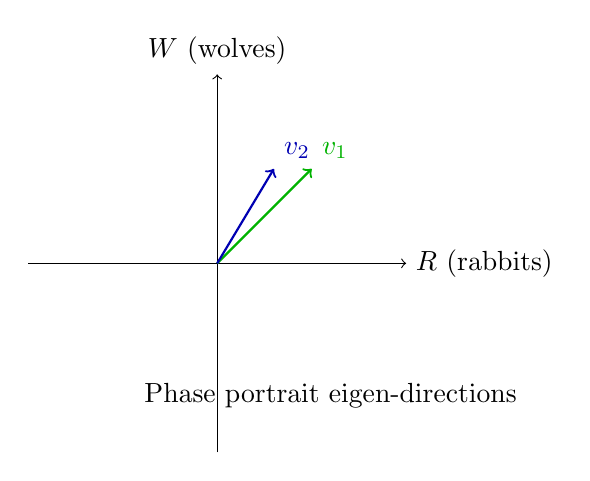
\begin{tikzpicture}[scale=1.2]
  \draw[->] (-2,0) -- (2,0) node[right]{$R$ (rabbits)};
  \draw[->] (0,-2) -- (0,2) node[above]{$W$ (wolves)};
  % eigenvector v1 (1,1)
  \draw[thick,green!70!black,->] (0,0) -- (1,1) node[above right]{$v_1$};
  % eigenvector v2 (3/5,1)
  \draw[thick,blue!70!black,->] (0,0) -- (0.6,1) node[above right]{$v_2$};
  \node at (1.2,-1.4) {Phase portrait eigen-directions};
\end{tikzpicture}
\end{frame}

% ---- Explanation slide ----
\begin{frame}{What the Graph Means}
\textbf{Explanation for the audience:}
\begin{itemize}
  \item The green and blue arrows show the main directions that the populations move along over time.
  \item Each arrow represents an \textbf{eigenvector}, or a special balance between wolves and rabbits.
  \item The slope of each arrow tells us how the two species change together — if rabbits increase, how wolves respond, and vice versa.
  \item As years go by, no matter where we start, the populations move closer to one of these directions.
  \item Because both eigenvalues are less than 1, all movements shrink toward the \textbf{origin (0,0)}, meaning both populations eventually decline to a stable point.
\end{itemize}
\end{frame}

\begin{frame}{General Solution and Long-Run Behavior}
  If $A$ is diagonalizable (it is), any initial state decomposes as $\vb x_0=c_1\vb v_1+c_2\vb v_2$ and
  \[
    \vb x_t=c_1\,\lambda_1^t\,\vb v_1 + c_2\,\lambda_2^t\,\vb v_2
    = c_1(0.7)^t\begin{bmatrix}1\\1\end{bmatrix} + c_2(0.9)^t\begin{bmatrix}3/5\\1\end{bmatrix}.
  \]
  Ratio of coordinates (wolves/rabbits):
  \[
    \frac{W_t}{R_t} = \frac{c_1(0.7)^t + \tfrac{3}{5}c_2(0.9)^t}{c_1(0.7)^t + c_2(0.9)^t}
    \xrightarrow[t\to\infty]{} \frac{3}{5},\quad \text{since }0.9>0.7.
  \]
  \textbf{Therefore:} trajectories decay to the origin (both eigenvalues $<1$), and their direction approaches the dominant eigenvector $\vb v_2=\begin{bmatrix}3/5\\1\end{bmatrix}$.
\end{frame}

\section{Equilibria Types}
\begin{frame}{Attractors, Repellors, Saddle Points}
  For a linear discrete system $\vb x_{t+1}=A\,\vb x_t$:
  \begin{itemize}
    \item If the spectral radius $\rho(A)<1$ (all eigenvalues have $|\lambda|<1$), the origin is a \textbf{(globally) asymptotically stable attractor}.
    \item If all eigenvalues have $|\lambda|>1$, the origin is a \textbf{repellor}.
    \item If some $|\lambda|<1$ and some $|\lambda|>1$, the origin is a \textbf{saddle point}.
    \item Complex eigenvalues yield \textbf{spirals/oscillations}; real eigenvalues yield \textbf{straight-line} approach along eigendirections.
  \end{itemize}
  In our model, $0.7,0.9<1$ $\Rightarrow$ origin is an attractor; approach is along $\vb v_2$.
\end{frame}

\section{Continuous-Time Contrast}
\begin{frame}{Lotka--Volterra (Continuous-Time)}
  The classical Lotka--Volterra system (differential equations) is
  \[
    \dv{x}{t}=ax-cxy,\qquad \dv{y}{t}=-by+dxy,\qquad a,b,c,d\ge0.
  \]
  Equilibria: $(0,0)$ and $(\tfrac{b}{d},\tfrac{a}{c})$.
  Jacobian:
  \[
    J(x,y)=\begin{bmatrix} a-cy & -cx\\ dy & dx-b\end{bmatrix},\quad
    J\!\left(\tfrac{b}{d},\tfrac{a}{c}\right)=\begin{bmatrix}0 & -\tfrac{bc}{d}\\ \tfrac{ad}{c} & 0\end{bmatrix}.
  \]
  The linearization has purely imaginary eigenvalues $\lambda=\pm i\sqrt{ab}$ (neutral center), so trajectories are closed orbits in the linear model (true nonlinear behavior depends on parameters and invariants).
\end{frame}

\section{Conclusion}
\begin{frame}{Conclusion}
  \begin{itemize}
    \item Eigenvalues/eigenvectors characterize long-run behavior of linear (and linearized) dynamical systems.
    \item In the discrete predator--prey example, both $|\lambda|<1$ $\Rightarrow$ populations decay to the origin; direction aligns with the dominant eigenvector.
    \item Linear tools also clarify stability of nonlinear models via linearization (e.g., Lotka--Volterra).
    \item Applications span signal processing, structural stability, control, and resource exploration.
  \end{itemize}
\end{frame}

\section{References}
\begin{frame}{References}
  \footnotesize
  \begin{itemize}
    \item Boyce \\ DiPrima notes on predator--prey (ODEs):\\ \url{https://faculty.etsu.edu/gardnerr/Differential-Equations/DE-BoyceDiprima5-notes/BoyceDiPrima5-9-7.pdf}
    \item UCI Math predator--prey notes:\\ \url{https://www.math.uci.edu/~ndonalds/math3d/predator.pdf}
    \item UBC predator--prey resources:\\ \url{https://personal.math.ubc.ca/~israel/m215/predprey/predprey.html}
    \item Caltech CDS notes on linear systems:\\ \url{https://www.cds.caltech.edu/~murray/courses/cds101/fa02/caltech/pph02-ch19-23.pdf}
    \item Discrete dynamical systems primer:\\ \url{https://personal.math.ubc.ca/~tbjw/ila/dds.html}
  \end{itemize}
\end{frame}

\end{document}
